\documentclass[a4paper,10pt]{article}
\usepackage[a4paper, margin=1in]{geometry}
\usepackage[utf8]{inputenc}
\usepackage{amsmath}
\usepackage{amssymb}
%\usepackage{physymb}
\usepackage{graphicx}
\graphicspath{{img/}}
\usepackage[font=scriptsize]{caption}
\usepackage{subfig}
\usepackage{float}
\usepackage{framed}
\usepackage{listings}
\usepackage{verbatim}
\usepackage{hyperref}
% make footnotes stick to the bottom
\usepackage[bottom]{footmisc}

% set code snippets to Python
\lstset{
frame=single,
language=Python, 
framexleftmargin=5pt,
basicstyle=\small\ttfamily,
showstringspaces=false
}

% remove paragraph indents
\setlength\parindent{0pt}

\newcommand\centerme[1]{\begin{center}#1\end{center}}

% this would be elegant but lstlisting requires some special handling and doesn't work
\newenvironment{commandexample}[1]
{\begin{tabular}{c}\begin{verbatim}[linewidth=#1, language=Python]{}}
{\end{verbatim}\end{tabular}}

\begin{document}

\begin{minipage}{0.30\textwidth}
%\begin{flushleft}
    %\begin{figure}[H]
    
\includegraphics[width=0.9\textwidth]{uds_logo.pdf}
    %\end{figure} 
    %\end{flushleft}
    %\vspace{0.01cm}
\end{minipage}
\begin{minipage}{0.69\textwidth} 
\vspace{0.2cm}
\begin{flushright}
\Large{\textbf{Statistical Natural Language Processing}} \\
\vspace{0.1cm}
\small{Summer Semester 2021} \\
\small{Prof. Dr. Dietrich Klakow} \\
\small{Tutors: Awantee Deshpande, Vilém Zouhar, Julius Steuer} \\
\end{flushright}
\end{minipage}

\vspace{1cm}

% A more elegant solution would be to use \maketitle and style it there
% though this is probably faster. -VZ
\centerme{
\Large{\textbf{Instructions for using Jupyter Notebooks and Assignments}}
}

For this course, all your assignments will be provided to you in the form of Jupyter Notebooks, and they must be submitted as Notebooks as well (unless mentioned otherwise). You can utilise either Google Colab for working on them with your teammate or install Jupyter Notebook on your local machine. Below, we provide you with some instructions to help you get started.

\section{Google Colab}
It is possible to create, upload, download, store, and share notebooks using Colab. You can also mount your Google Drive to use the data stored there. These notebooks can also be downloaded as .py files and PDFs.

\subsection{Getting started}
\begin{enumerate}
    \item To use Colab, you need to have a Google account. Go to \href{https://colab.research.google.com}{\nolinkurl{colab.research.google.com}} and sign in with your Google account. A folder called `Colab Notebooks' will be created in your Drive. 
    \item You can create a new Notebook by clicking \texttt{File $\rightarrow$ New Notebook} on the Colab website, or from your Drive by selecting \texttt{New $\rightarrow$ More $\rightarrow$ Google Colaboratory}.
    
    \item You can rename your Notebook in the top left corner:
    
    \begin{center}
    \fbox{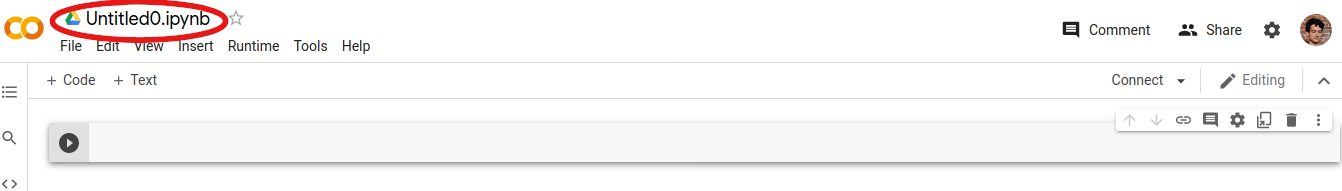
\includegraphics[width=0.95\linewidth]{new_notebook.png}}
    \end{center}
\end{enumerate}

\subsection{Other functionality}
\begin{enumerate}
    \item You can change the Runtime by clicking on \texttt{Runtime $\rightarrow$ Change runtime type} and select the appropriate runtime and hardware accelerator. (Not required at the moment.)
    
    \item \textbf{Mounting the Drive}: You can use the data stored on the Drive by mounting it in your Colab environment. To do this, either run the following command in your Notebook cell
    
\begin{center}
\begin{tabular}{l}
\begin{lstlisting}[linewidth=6.5cm]
from google.colab import drive
drive.mount(`/content/gdrive')
\end{lstlisting}
\end{tabular}
\end{center}
    
    Or, you can simply select the folder icon as shown below and mount the drive:
    
    \begin{center}
    \fbox{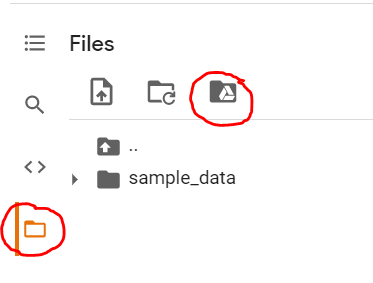
\includegraphics[width=0.25\linewidth]{mount_drive.PNG}}
    \end{center}
    
    \newpage
    \item Most system based commands can be directly run from the Notebook by prepending them with an `!' symbol. This allows on-the-fly installation and cloning functionalities.
    
\begin{center}
\framebox{\texttt{!pip install numpy}}
\end{center}
    
    \item For further details and usage, refer to \\
    \small \href{https://www.analyticsvidhya.com/blog/2020/03/google-colab-machine-learning-deep-learning/}{\nolinkurl{analyticsvidhya.com/blog/2020/03/google-colab-machine-learning-deep-learning/}}
\end{enumerate}

\section{Local Machine}
You can also use Jupyter Notebooks on your local machine. To do this, follow the given steps:

\subsection{Set up Anaconda}
\label{subsec:local}
Most installations recommend using the conda package manager which makes it easy to set up environments and install all necessary packages.
For this, you need to download and install Anaconda.\footnote{\href{https://www.anaconda.com/products/individual}{\nolinkurl{anaconda.com/products/individual}}} \\
Note that you need to use the Anaconda prompt if you're using Windows, or make sure you add the Anaconda file path to your system environment variables.\\
Launch Jupyter Notebook in the current file path by typing:

\begin{center}
\framebox{\texttt{\$ jupyter notebook}}
\end{center}

This will open a new Jupyter Notebook instance in your browser. All the files in your current directory will be visible in this instance.

\subsection{Set up conda environment}
Since you might require specific packages and versions for your assignments, we recommend that you create a separate environment for this course. Specify the base packages while creating your environment:

\begin{center}
\framebox{\texttt{\$ conda create -n snlp python=3.7 numpy matplotlib}}
\end{center}

Or, you can install packages separately in your environment using the command
\begin{center}
\framebox{\texttt{\$ conda install <package-name>}}
\end{center}

You can activate / deactivate your environment with the commands
\begin{center}
\framebox{\texttt{\$ source activate snlp}}
\end{center}
\begin{center}
\framebox{\texttt{\$ source deactivate}}
\end{center}

To add your environment to your Jupyter Notebook, you need to install ipykernel using
\begin{center}
\framebox{\texttt{\$ conda install -c anaconda ipykernel}}
\end{center}

After installing, just run
\begin{center}
\framebox{\texttt{\$ python -m ipykernel install --user --name=snlp}}
\end{center}

You can now create a new Notebook in that environment:

\begin{center}
\fbox{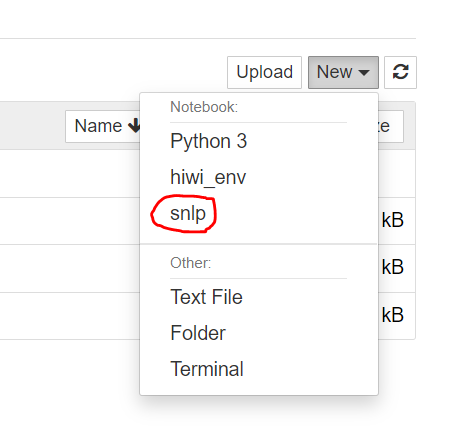
\includegraphics[width=0.22\linewidth]{add_env.PNG}}
\end{center}

\section{Importing Python code in Notebook}

We mostly require you to answer only textually in the notebook and to store your Python code in pure \texttt{.py} files. For that, you have to import the file and call the functions from the Notebook.
If your Python file is saved in a directory other than your current directory, you can import it to your Notebook by adding it to your system path:

\begin{center}
\fbox{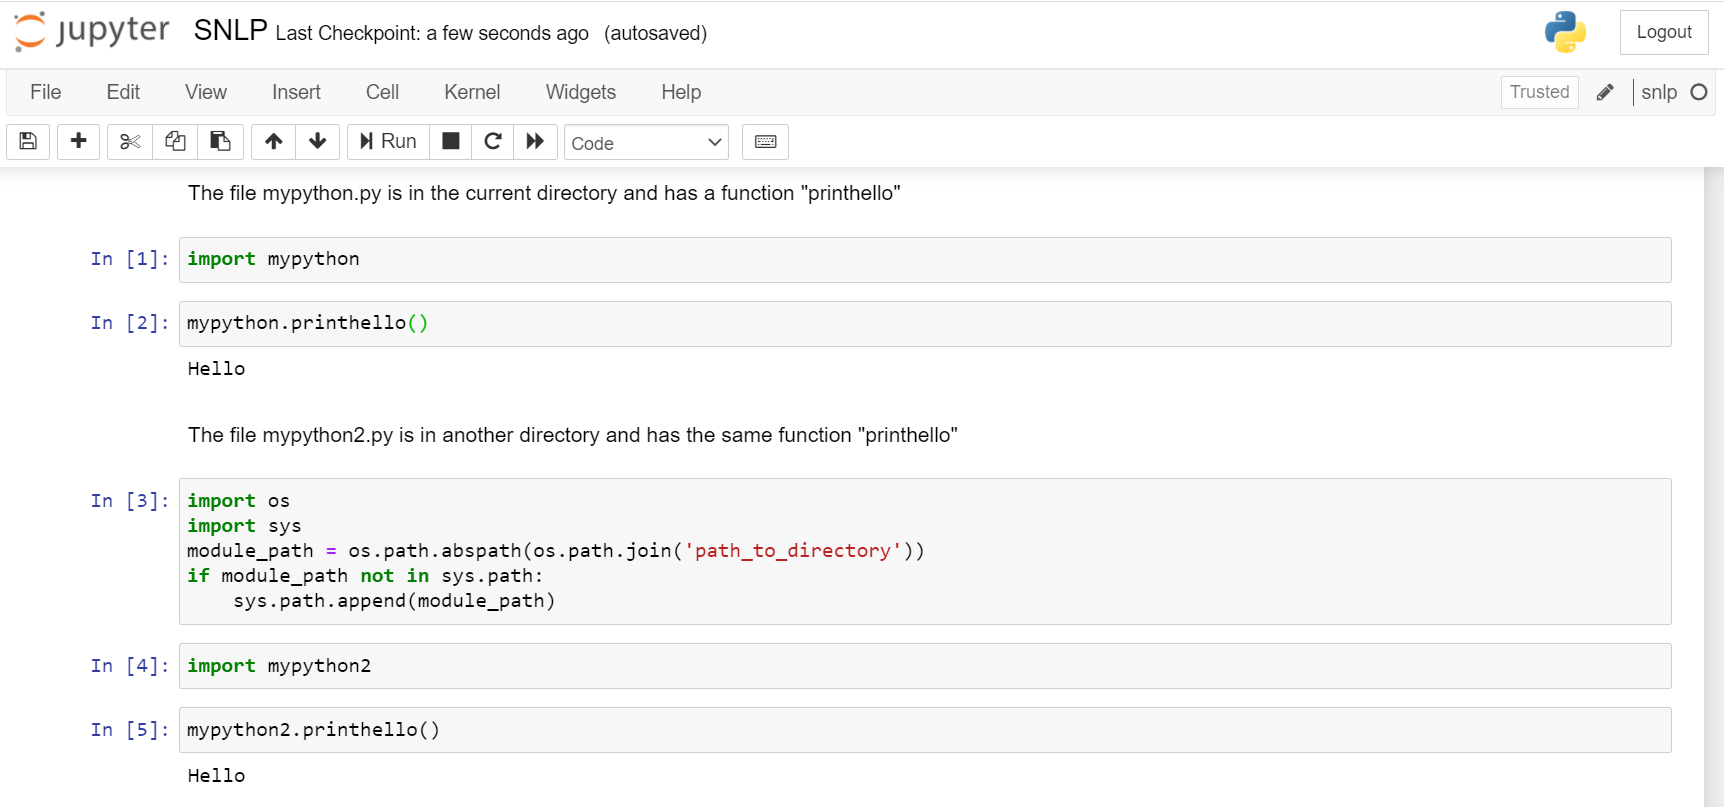
\includegraphics[width=0.95\linewidth]{import_py.PNG}}
\end{center}

However, once your Python file has been imported into the Notebook, if you make changes to this code, the Notebook does not reimport these changes. One way to overcome this is to restart the kernel and rerun the Notebook cells. Another way is to utilise Python's importlib module in the Notebook as follows:

\begin{center}
\begin{tabular}{c}
\begin{lstlisting}[linewidth=7.5cm]
from importlib import reload
import mypython2
mypython2 = reload(mypython2)
\end{lstlisting}
\end{tabular}
\end{center}

You can also connect Google Colab to your local runtime, which allows you to execute code on your local hardware and have access to your local file system. For this, you need to install Jupyter to your local machine, as indicated in Section \ref{subsec:local}.

\begin{enumerate}
    \item You also need to install and enable the \texttt{ jupyter\_http\_over\_ws} Jupyter extension.
    
\begin{lstlisting}[linewidth=12cm, language=Python]
$ pip install jupyter_http_over_ws
$ jupyter serverextension enable --py jupyter_http_over_ws
\end{lstlisting}

    \item To start the server, you need to need to set a flag to explicitly trust WebSocket connections from the Collaboratory frontend.
 
\begin{lstlisting}[linewidth=13cm]
$ jupyter notebook \
--NotebookApp.allow_origin=`https://colab.research.google.com' \
--port=8888 \
--NotebookApp.port_retries=0
\end{lstlisting}
\end{enumerate}

\section{Other functionalities of Notebooks}
For most assignments, you will be required to write a text-based answer or analysis along with the coding solution. To avoid utilising multiple file formats, you are expected to write your analyses in the same Notebook. For this, we ask you to get acquainted with certain other features provided by Jupyter Notebooks, such as using Markdown for text, LaTeX for mathematical equations etc.\\

This can be done in Google Colab by simply creating the cell as a \texttt{Text} cell instead of a \texttt{Code} cell. In your local runtime, you can toggle the cell type in the dropdown menu. \\

\begin{figure}[H]
    \centering
    \subfloat[Google Colab]{\fbox{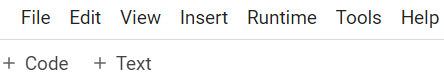
\includegraphics[width=0.35\textwidth]{code_text.PNG}}}
    \hspace{1em}
    \subfloat[Local Notebook]{\fbox{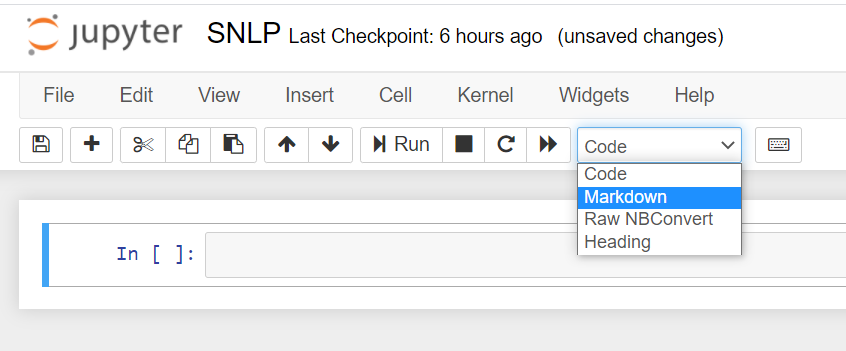
\includegraphics[height=3cm]{markdown.png}}}
\end{figure}

An example of markdown and LaTeX renderings in the code cell:

\begin{center}
\fbox{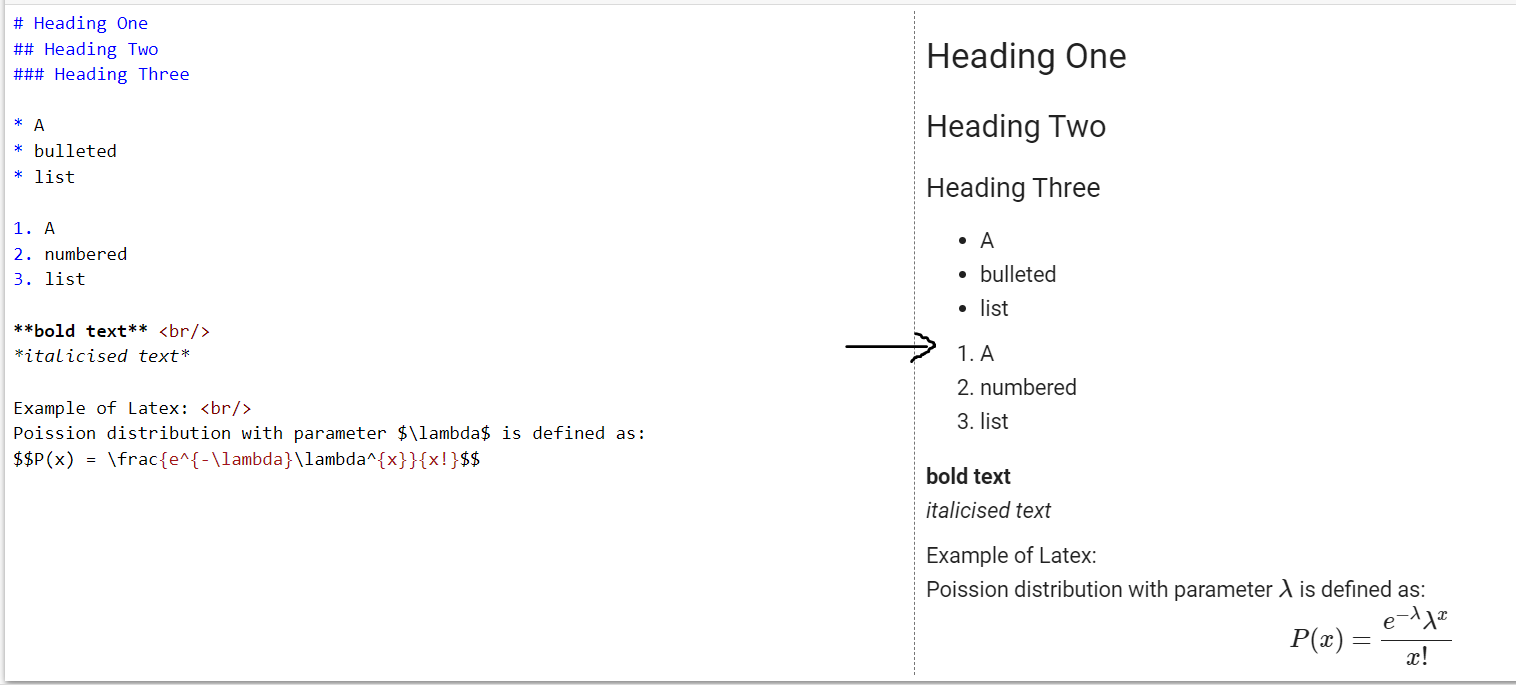
\includegraphics[width=0.95\linewidth]{render_text.PNG}}
\end{center}

Please refer to the following link for more examples:

\small \href{https://towardsdatascience.com/write-markdown-latex-in-the-jupyter-notebook-10985edb91fd}{\nolinkurl{towardsdatascience.com/write-markdown-latex-in-the-jupyter-notebook-10985edb91fd}}

\section{Submission}
As you will be working in teams of two, please name your Notebook submission in the format:

\begin{center}
\fbox{\texttt{Name1\_id1\_Name2\_id2.ipynb}}
\end{center}

Wherever you have to submit more than one file, you should place them all in one folder and submit the zipped contents. The submitted folder should also follow the same naming template. 
\textbf{If you do not follow the formal requirements, the tutors can decide not to grade your submission.} \\

You will be explicitly informed separately in each assignment what files to submit, and what format they should adhere to. Please make sure you follow those instructions consistently across all the assignment submissions. Also, when you submit your assignments in Teams, you must remember to upload the submission \textbf{AND} click on the ``Turn-in" button at the top right hand corner. Otherwise your assignment will not be considered as submitted. \\

Assignments will be released at 23:59 on the day of the lecture (i.e. every Friday). This is also the deadline for the previous week's assignment.\\

If you have any problems with your system setup, as well as clarifications about the assignments, first check Piazza\footnote{\href{https://piazza.com/class?nid=kniwgq42qek5oe}{\nolinkurl{piazza.com/class?nid=kniwgq42qek5oe}}} for similar posts, and only then create a new question, which we will do our best to answer as soon as possible. You are free (and encouraged) to answer other people's questions if you know the answer.

\end{document} 